\begin{frame}
	\begin{fancycolumns}[height=8.5cm,reverse]
		\pic[width=\linewidth,trim=0 240 0 300,clip]{people/andy-hunt}
		\vspace{-7mm}
		
		\begin{note}{Andy Hunt \mysource{\thepragmaticprogrammer}}
			\mycite{No one in the brief history of computing has ever written a piece of perfect software. It's unlikely that you'll be the first.}
		\end{note}
		% co-authored The Pragmatic Programmer, known for the Agile Manifesto
		\nextcolumn
		\pic[width=\linewidth,trim=425 0 400 0,clip]{people/donald-trump}
		\vspace{-7mm}
		
		\begin{note}{Donald Trump (May 2020) \mysource{\href{https://www.huffpost.com/entry/trump-testing-claim-pennsylvania_n_5ebdf19bc5b6c9c187419778}{huffpost.com}}}
			\mycite{If we didn’t do any testing, we would have very few cases.}
		\end{note}
	\end{fancycolumns}
\end{frame}

\subsection{Software Quality}
\begin{frame}{\insertsubsection}
	\begin{fancycolumns}
		\begin{definition}{Quality \mysource{\ludewiglichter}}
			Quality is the entirety of properties and characteristics of a product or process that indicate adequacy with respect to given requirements.
		\end{definition}
		\begin{definition}{Quality Assurance \mysource{\ludewiglichter}}
			Quality assurance \deutsch{Qualitätssicherung} are all activities with the goal to improve the quality.
		\end{definition}
		\nextcolumn
		\begin{note}{Expectations on Quality \mysource{\sommerville}}
			\mycite{Because of their previous experiences with buggy, unreliable software, users sometimes have low expectations of software quality. They are not surprised when their software fails. When a new system is installed, users may tolerate failures because the benefits of use outweigh the costs of failure recovery. However, as a software product becomes more established, users expect it to become more reliable.\uncover<3->{ [...] If a software product or app is very cheap, users may be willing to tolerate a lower level of reliability.}\uncover<4->{ [...] Customers may be willing to accept the software, irrespective of problems, because the costs of not using the software are greater than the costs of working around the problems.}}
		\end{note}
	\end{fancycolumns}
\end{frame}

\subsection{Product Quality}
\begin{frame}[label=productquality]{\insertsubsection\ \mytitlesource{\isoiectfzoz}}
	\label{slide:productquality}
	\vspace{-9mm}
	\hfill
	\begin{tikzpicture}
		\path[small mindmap,
		every node/.style={concept,font=\scriptsize},
		emph/.style={font=\bfseries\scriptsize},
		hide/.style={visible on=<1->},
		concept color=foreground!20!background,
		level 1/.append style={level distance=25mm,sibling angle=360/8},
		level 2/.append style={level distance=20mm,sibling angle=360/12},
		level 3/.append style={level distance=20mm,sibling angle=360/8},
		]
		node {Product Quality \deutsch{Produktqualität}}
		[clockwise from=0]
		child[concept color=orange!20!background,visible on={<5,7>},level distance=33mm] { node {Maintainability} 
			[clockwise from=30]
			child { node {Modularity} }
			child { node {Reusability} }
			child { node {Analysability} }
			child { node {Modifyability} }
			child { node {Testability} }
		}
		child[concept color=red!20!background,visible on={<4,7>}] { node {Performance Efficiency ...} }
		child[concept color=blue!20!background,visible on={<4,7>}] { node {Compatibility ...} }
		child[concept color=green!20!background,visible on={<4,7>}] { node {Usability ...} }
		child[concept color=red!20!background,visible on={<3,7>},level distance=28mm] { node {Reliability} 
			[clockwise from=255]
			child { node {Maturity} }
			child { node {Availability} }
			child { node {Fault Tolerance} }
			child { node {Recoverability} }
		}
		child[concept color=orange!20!background,visible on={<2,7>}] { node {Security} 
			[clockwise from=190]
			child { node {Confidentiality} }
			child { node {Integrity} }
			child { node {Non-Repudiation} }
			child { node {Accountability} }
			child { node {Authenticity} }
		}
		child[concept color=green!20!background,visible on={<1,7>}] { node {Functional Suitability} 
			[clockwise from=90]
			child { node {Completeness} }
			child { node {Correctness} }
			child { node {Appropriateness} }
		}
		child[concept color=blue!20!background,visible on={<6-7>}] { node {Portability} 
			[clockwise from=50]
			child { node {Adaptability} }
			child { node {Installability} }
			child { node {Replaceability} }
		}
		;
	\end{tikzpicture}
	\hspace{-5mm}
\end{frame}
% omitted categories:
%   performance efficiency: time behaviour, resource utilization, capacity
%   compatibility: co-existence, interoperability
%   usability: appropriateness recognizability, learnability, operability, user error protection,
%              user interface aesthetics, accessibility

\subsection{Quality in Use}
\begin{frame}{\insertsubsection\ \mytitlesource{\isoiectfzoz}}
	\begin{tikzpicture}
		\path[small mindmap,
		every node/.style={concept,font=\scriptsize},
		emph/.style={font=\bfseries\scriptsize},
		hide/.style={visible on=<1->},
		concept color=foreground!20!background,
		level 1/.append style={level distance=25mm,sibling angle=360/7},
		level 2/.append style={level distance=20mm,sibling angle=360/11},
		level 3/.append style={level distance=20mm,sibling angle=360/8},
		]
		node {Quality in Use \deutsch{Gebrauchsqualität}}
		[clockwise from=193]
		child[concept color=blue!20!background,visible on={<1,5>}] { node {Effectiveness} }
		child[concept color=blue!20!background,visible on={<1,5>}] { node {Efficiency} }
		child[concept color=green!20!background,visible on={<2,5>}] { node {Satisfaction} 
			[clockwise from=155]
			child { node {Usefulness} }
			child { node {Trust} }
			child { node {Pleasure} }
			child { node {Comfort} }
		}
		child[concept color=red!20!background,visible on={<3,5>}] { node {Freedom from Risk} 
			[clockwise from=75]
			child { node {Economic Risk Mitigation} }
			child { node {Health and Safety Risk Mitigation} }
			child { node {Environmental Risk Mitigation} }
		}
		child[concept color=orange!20!background,visible on=<4-5>] { node {Context Coverage} 
			[clockwise from=30]
			child { node {Context Completeness} }
			child { node {Flexibility} }
		}
		;
	\end{tikzpicture}
\end{frame}

\xkcdframe{2200} % unreachable state

\subsection{Software Testing}
\begin{frame}{\insertsubsection}
	\begin{fancycolumns}[height=1cm,animation=none]
		\uncover<1->{
			\begin{definition}{Software Testing \mysource{\sommerville}}
				\mycite{Testing is intended to show that a program does what it is intended to do and to discover program defects before it is put into use.}
			\end{definition}
		}
		\uncover<2->{
			\begin{definition}{Validation Testing \mysource{\sommerville}}
				\mycite{Demonstrate to the developer and the customer that the software meets its requirements.}
			\end{definition}
		}
		\uncover<3->{
			\begin{definition}{Defect Testing \mysource{\sommerville}}
				\mycite{Find inputs or input sequences where the behavior of the software is incorrect, undesirable, or does not conform to its specification.}
			\end{definition}
		}
		\nextcolumn
		%\vspace{-12mm}
		\uncover<4->{
			\begin{note}{V\&V \mysource{\seeconomics}}
				\mycite{\emph{Validation}: Are we building the right product?\\\emph{Verification}: Are we building the product right?}
			\end{note}	
		} 
		% TODO better visualization of V&V (see Inas slides). move to V model?
		\vspace{-.7mm}
		\uncover<5->{
			\begin{note}{Stages of Testing \mysource{\sommerville}}
				\begin{itemize}
					\setlength\itemsep{.1em}
					\item[1.] \mycite{\emph{Development testing}, where the system is tested during development to discover
						bugs and defects}
					\item[2.] \mycite{\emph{Release testing}, where a separate testing team tests a complete version of the
						system before it is released to users}
					\item[3.] \mycite{\emph{User testing}, where users or potential users of a system test the system in their
						own environment}
				\end{itemize}
			\end{note}
		}
		\vspace{-.7mm}
		\uncover<6->{
			\begin{note}{}
				\mycite{In \emph{manual testing}, a tester runs the program with some test data and
					compares the results to their expectations. [...] In \emph{automated testing}, the tests are encoded in a program that is run each time the system under development is to be tested.} \mysource{\sommerville}
			\end{note}
		}
	\end{fancycolumns}
\end{frame}

\subsection{Quality Assurance}
\begin{frame}{\insertsubsection\ \mytitlesource{\ludewiglichter}}
	\slideMindmapQualityAssurance{}{}{}{visible on={<2->}}{visible on={<4->}}{visible on={<5->}}{visible on={<3->}}
\end{frame}

\subsection{Code Reviews} % TODO add literature on code reviews
\begin{frame}{\insertsubsection}
	\begin{fancycolumns}
		\begin{definition}{}
			\begin{itemize}
				\item Idea: improve quality by asking other programmers for feedback
				\item Typically applied with quality checklist
				\item Quality criteria: functionality, comprehensibility, maintainability, coding guidelines, design patterns, \ldots
				\item Reviewer selection: based on familiarity with code, availability, expertise
			\end{itemize}
		\end{definition}
		\pic[width=\linewidth,trim=0 40 0 10,clip]{codereview/codereview1}
		\nextcolumn
		\begin{note}{}
			\begin{itemize}
				\item Cannot be done by yourself
				\item Reviewers need programming experience and knowledge of the code (mutual feedback)
				\item Feedback should be timely and constructive
				\item Only changes reviewed, not too many
			\end{itemize}
		\end{note}
		\uncover<3->{\pic[width=.49\linewidth,trim=83 0 210 0,clip]{codereview/codereview3}}\hfill
		\uncover<4->{\pic[width=.49\linewidth,trim=50 0 450 0,clip]{codereview/codereview2}}
	\end{fancycolumns}
\end{frame}

\begin{frame}{\insertsubsection\ on Github}
	\picDark[width=\linewidth]{../pics/codereview/github}
	%\href{https://github.com/tthuem/FeatureIDE/commit/73df3fd463487c3adb17ca9cb39ba647deddc5ba}{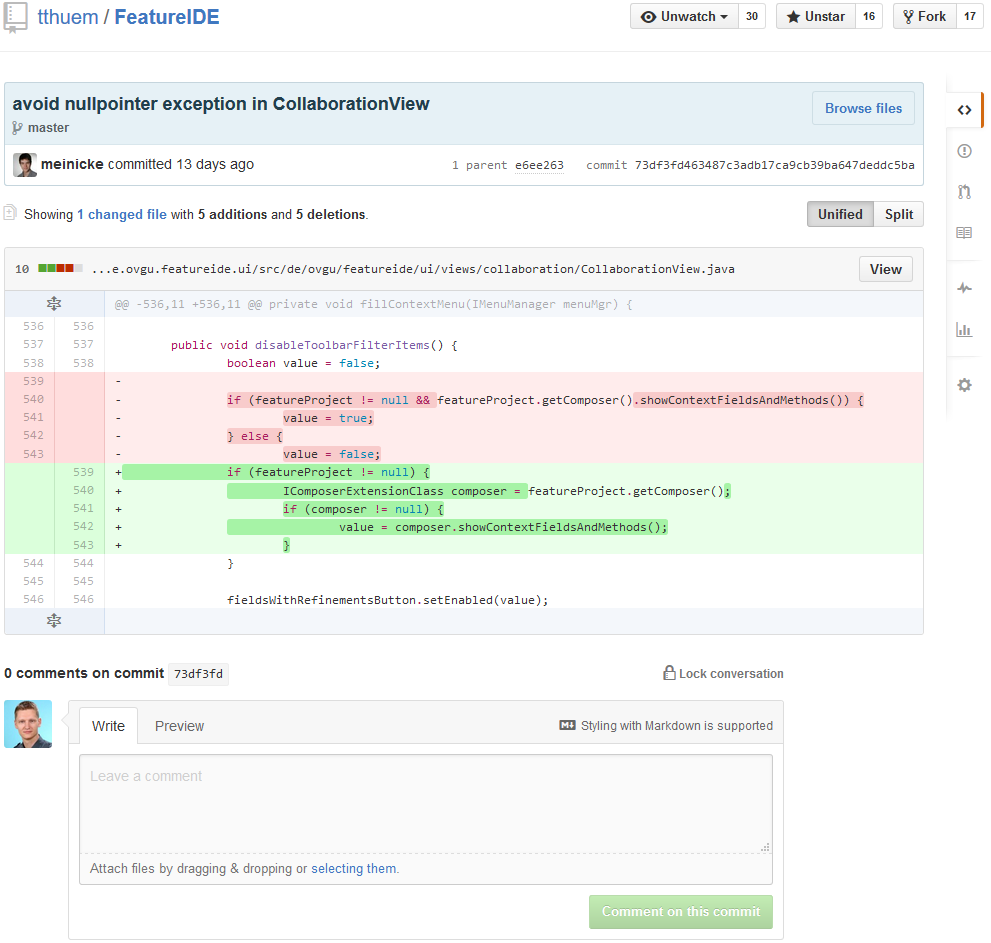
\includegraphics[height=.9\textheight]{../pics/codereview/github2}}
\end{frame}
